\documentclass[12pt]{standalone}
\usepackage{tikz}
\usepackage{float}
\usepackage{pgfplots}
\usepackage{amsmath, amsfonts, amssymb}
\usetikzlibrary{shapes.geometric, arrows}

\tikzstyle{node} = [rectangle]

\newcommand{\comment}[1]{}

% 128K on 2080
\begin{document}
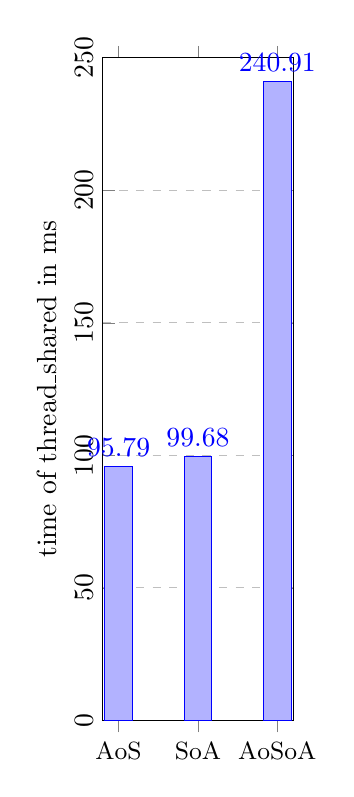
\begin{tikzpicture}
	\begin{axis}[
		%ybar, ymin=0,
		width=4cm, height=10cm,
		ylabel={time of thread\_shared in ms},
		symbolic x coords={AoS, SoA, AoSoA},
		xtick=data,
		yticklabel style={rotate=90},
		ymin=0, ymax=250,
		ytick={0,50,100,150,200,250},
		ybar=5pt,
		ymajorgrids=true,
		grid style=dashed,
		nodes near coords,
		x tick label style={font=\small,text width=1cm,align=center}
		]
		
    \addplot%+[only marks, mark=-]
    	coordinates {    		
    		(AoS, 95.79)
    		(SoA, 99.68)
    		(AoSoA, 240.91)
    	};
  \end{axis}
\end{tikzpicture}
\end{document}